
\documentclass[10pt,a4paper]{article}
\usepackage[T1]{fontenc}
\usepackage{tikz}
\usepackage[margin=1cm]{geometry}
\begin{document}
\section*{Final Tree:}
% Section title for the final binary search tree
\section*{Final Binary Search Tree}
% Explanation of what the document contains
This document presents the final binary search tree (BST) after performing a series of node deletions. The BST maintains its properties, where each node has a left child with a smaller value and a right child with a larger value.

% Subsection explaining the deletion algorithm used
\subsection*{Deletion Algorithm}
The following algorithm was used to delete nodes from the binary search tree:
\begin{center}
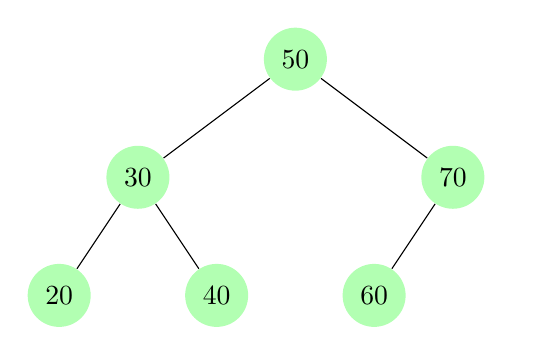
\begin{tikzpicture}[level distance=15mm, sibling distance=20mm]
    \tikzstyle{every node}=[circle,inner sep=1pt, minimum size=8mm]
    \tikzstyle{level 1}=[sibling distance=40mm]
    \tikzstyle{level 2}=[sibling distance=20mm]
    \tikzstyle{level 3}=[sibling distance=15mm]
    \tikzstyle{level 4}=[sibling distance=10mm]
    \node [fill=green!30] {50} child {node [fill=green!30] {30} child {node [fill=green!30] {20} } child {node [fill=green!30] {40} }} child {node [fill=green!30] {70} child {node [fill=green!30] {60} } child[fill=none] {edge from parent[draw=none]}};

\end{tikzpicture}
\end{center}
\end{document}
